\documentclass[12pt,]{article}
\usepackage{lmodern}
\usepackage{amssymb,amsmath}
\usepackage{ifxetex,ifluatex}
\usepackage{fixltx2e} % provides \textsubscript
\ifnum 0\ifxetex 1\fi\ifluatex 1\fi=0 % if pdftex
  \usepackage[T1]{fontenc}
  \usepackage[utf8]{inputenc}
\else % if luatex or xelatex
  \ifxetex
    \usepackage{mathspec}
  \else
    \usepackage{fontspec}
  \fi
  \defaultfontfeatures{Ligatures=TeX,Scale=MatchLowercase}
    \setmonofont[Mapping=tex-ansi]{Times New Roman}
\fi
% use upquote if available, for straight quotes in verbatim environments
\IfFileExists{upquote.sty}{\usepackage{upquote}}{}
% use microtype if available
\IfFileExists{microtype.sty}{%
\usepackage{microtype}
\UseMicrotypeSet[protrusion]{basicmath} % disable protrusion for tt fonts
}{}
\usepackage[margin=1in]{geometry}
\usepackage{hyperref}
\hypersetup{unicode=true,
            pdfborder={0 0 0},
            breaklinks=true}
\urlstyle{same}  % don't use monospace font for urls
\usepackage{longtable,booktabs}
\usepackage{graphicx,grffile}
\makeatletter
\def\maxwidth{\ifdim\Gin@nat@width>\linewidth\linewidth\else\Gin@nat@width\fi}
\def\maxheight{\ifdim\Gin@nat@height>\textheight\textheight\else\Gin@nat@height\fi}
\makeatother
% Scale images if necessary, so that they will not overflow the page
% margins by default, and it is still possible to overwrite the defaults
% using explicit options in \includegraphics[width, height, ...]{}
\setkeys{Gin}{width=\maxwidth,height=\maxheight,keepaspectratio}
\setlength{\emergencystretch}{3em}  % prevent overfull lines
\providecommand{\tightlist}{%
  \setlength{\itemsep}{0pt}\setlength{\parskip}{0pt}}
\setcounter{secnumdepth}{5}
% Redefines (sub)paragraphs to behave more like sections
\ifx\paragraph\undefined\else
\let\oldparagraph\paragraph
\renewcommand{\paragraph}[1]{\oldparagraph{#1}\mbox{}}
\fi
\ifx\subparagraph\undefined\else
\let\oldsubparagraph\subparagraph
\renewcommand{\subparagraph}[1]{\oldsubparagraph{#1}\mbox{}}
\fi

%%% Use protect on footnotes to avoid problems with footnotes in titles
\let\rmarkdownfootnote\footnote%
\def\footnote{\protect\rmarkdownfootnote}

%%% Change title format to be more compact
\usepackage{titling}

% Create subtitle command for use in maketitle
\providecommand{\subtitle}[1]{
  \posttitle{
    \begin{center}\large#1\end{center}
    }
}

\setlength{\droptitle}{-2em}

  \title{}
    \pretitle{\vspace{\droptitle}}
  \posttitle{}
    \author{}
    \preauthor{}\postauthor{}
    \date{}
    \predate{}\postdate{}
  
\usepackage{setspace}
\doublespacing

\begin{document}

\hypertarget{characterizing-the-secret-diets-of-siphonophores-cnidaria-hydrozoa-using-dna-metabarcoding}{%
\section{Characterizing the Secret Diets of Siphonophores (Cnidaria: Hydrozoa) using DNA Metabarcoding}\label{characterizing-the-secret-diets-of-siphonophores-cnidaria-hydrozoa-using-dna-metabarcoding}}

Authors (order TBD): Alejandro Damian-Serrano, Elizabeth Hetherington, Anela Choy, Steven Haddock, Alexandra Lapides, Casey Dunn

Alejandro Damian-Serrano\textsuperscript{1,‡}, Steven H.D. Haddock\textsuperscript{2}, Casey W. Dunn\textsuperscript{1}

\textsuperscript{1} Yale University, Department of Ecology and Evolutionary Biology, 165 Prospect St., New Haven, CT 06520, USA

\textsuperscript{2} Monterey Bay Aquarium Research Institute, 7700 Sandholdt Rd., Moss Landing, CA 95039, USA

MEPS Lim. 12K words

\newpage

\hypertarget{abstract}{%
\subsection*{Abstract}\label{abstract}}
\addcontentsline{toc}{subsection}{Abstract}

Siphonophores are abundant and diverse predators in the open-ocean ecosystems. Due to limited access to the deep midwater environment, little is known about the diets of most deep-dwelling species. Early work on the diets of epipelagic siphonophore species relied on visual gut content inspection, which can rarely detect and identify soft-bodied prey which does not leave recognizable parts behind. For deep-sea species, submersible observations are unable to identify small prey items (such as copepods, ostracods, and larval fish) through video recordings. Recently, the application of DNA metabarcoding in other marine predators has revealed the importance of prey taxa that were overlooked by visual methods. Moreover, metabarcoding can detect prey that was ingested hours before specimen collection from traces of DNA released during digestion and thus is better suited for the study of deep-sea species with long intervals between prey captures. In this study, we perform DNA metabarcoding analyses on the gut contents of several siphonophore species across the water column and describe their diets. We collected siphonophore specimens using blue water dives and ROV dives in open-ocean waters. We extracted DNA from the feeding bodies, then amplified and sequenced six barcode markers along the 18S gene. Taxonomic identifications were assigned to prey OTUs using SILVA databases combined with local zooplankton sequences. We find that most of the species analyzed here are specialized and strongly selective predators. Many of the interactions detected by our metabarcoding analyses are congruent with tentilla morphology-based predictions. In addition, our analyses were able to detect small prey and gelatinous prey taxa underrepresented by visual methods. Our results reveal hidden links between siphonophores and lower trophic levels in the midwater food-web. This study expands our understanding of the role of siphonophores in the open ocean, and the importance of their species diversity for nutrient flow and ecosystem functioning.

Lim. 250 words

\hypertarget{keywords}{%
\subsection*{Keywords}\label{keywords}}
\addcontentsline{toc}{subsection}{Keywords}

Siphonophore, trophic ecology, prey selectivity, DNA metabarcoding

\hypertarget{introduction}{%
\subsection*{Introduction}\label{introduction}}
\addcontentsline{toc}{subsection}{Introduction}

The open-ocean midwater is the largest volume of the biosphere habitable by animals (Harbison 1992). This environment hosts diverse communities and complex food webs (Robison 2004). Midwater food webs sustain manifold fisheries, charismatic megafauna, and sustain the biological carbon pump. Gelatinous animals play fundamental roles in these food webs (Choy et al. 2017), acting as herbivores, predators, and prey in the `jelly web' (Robison 2004, Chi et al. 2020). Among the most important gelatinous predators are siphonophores, mid-trophic predators that feed on a broad variety of prey taxa such as medusae, salps, crustaceans, molluscs, and fishes (Purcell 1981a, Hetherington et al. 2021). Siphonophores are sit-and-wait, non-visual, ambush predators that rely on prey coming into contact with the tentacles and tentilla (Mackie et al. 1988). They are abundant and locally diverse colonial cnidarians in open-ocean communities, present in every ocean of the world, with species ranging from the surface (like the Portuguese man-o-war) to the abyssopelagic region (\textgreater{}4000m deep) (Mapstone 2014). In addition, siphonophore aggregations can have significant predatory impacts on larval fish stocks (Purcell 1981b).

Progress in elucidating siphonophore diets has been slow due to the intrinsic challenges of working with these animals. Oceanic taxa require expensive research vessels to reach their habitat. In addition, siphonophores are extremely fragile creatures, requiring the use of blue water SCUBA divers and ROVs to collect them alive and intact (Haddock 2004). Traditional collection methods such as plankton nets not only break up the colonies, but also lead to artifactual ingestions in the cod-end that confound their natural diets. The diets of some epipelagic and siphonophore species are well known through gut content analyses of SCUBA-collected colonies (Biggs 1977, Purcell 1981a, reviewed in Hetherington et al. 2021). Recent studies based on ROV observations have shed some light on the diets of deep midwater siphonophores (Choy et al. 2017, Hetherington et al. 2021, Lapides \& others 2021). However, both of these approaches have been limited by their biases. Visual gut content inspection only recognizes hard-bodied prey that digest slowly, leaving behind diagnostic body parts (i.e.~exoskeleton, shell, eyes\ldots{}). Therefore, these methods are biased against soft-bodied, rapidly-digested taxa, such as gelatinous plankton. ROVs are able to observe feeding on gelatinous prey before it becomes digested. However, ROV observations are skewed towards large prey items that can be easily identified from the camera screen (such as jellyfish, shrimps, or fish), thus overlooking important prey items such as copepods and larvae (Hetherington et al. 2021). In addition, prey are scarce in the open ocean, especially in the deeper regions (Robison 2004), thus it is relatively rare to find specimens capturing prey or carrying visually-identifiable prey in the guts.

With the advent of DNA metabarcoding, the diets of many marine predators have been elucidated from gut content DNA (Leray et al. 2013, Harms-Tuohy et al. 2016, Fernández-Álvarez et al. 2018, Reis et al. 2018 ). These high-throughput amplicon sequencing technologies have extremely high detection sensitivity and bypass the biases posed by visual methods. In the past few years, the application of DNA metabarcoding to marine predator gut contents has demonstrated the capacity of these methods to detect gelatinous prey (Connell et al. 2014, McInnes et al. 2017, Clarke et al. 2018, Jensen et al. 2018, Marques et al. 2019). However, this technology has not yet been applied to study the diets of gelatinous animals.

In Hetherington et al. Hetherington et al. (2021), we reviewed and summarized the literature on siphonophore diets, and observed significant differences between the diets of epipelagic and deep-swelling siphonophore species. Gelatinous prey appeared to be more prevalent in deep-sea observations while small crustaceans appeared to be the predominant prey in shallow gut content samples. Since epipelagic species' diets were exclusively assessed through microscopic gut content inspection and deep-sea species' diets through ROV observations, it is not possible to determine whether these differences are due to ecological or methodological reasons. In order to disentangle these confounding factors, it is critical to assess both shallow and deep species' diets under the same methodological framework. In this case, DNA metabarcoding is an ideal choice, since it is able to detect both small and gelatinous prey, thus being able to bridge across the methodological shortcomings of visual methods.

In Damian-Serrano et al. Damian-Serrano \& Dunn (2022), we generated feeding guild predictions for 45 understudied siphonophore species using the discriminant analysis of principal components (DAPC) functions generated from the analyses in (Damian-Serrano et al. 2021). These analyses captured the complex multivariate relationships between tentilla and nematocyst morphology and feeding guild (based on published dietary assessments for 22 species). These predictions remain to be tested with new data on siphonophore diets.

Here we use DNA metabarcoding to identify the gut contents of several siphonophore species to obtain insights into their diets. The primary aims of this study are: (1) Expand the existing knowledge on the diets of open-ocean siphonophores using DNA metabarcoding, (2) compare the prey detected by visual and molecular methods to evaluate their technical biases, (3) compare the prey found in the gut contents to the local planktonic community composition to identify instances of selectivity and specialization, and (4) evaluate the morphology-based predictions of feeding guild generated in Damian-Serrano et al. Damian-Serrano \& Dunn (2022).

\hypertarget{methods}{%
\subsection*{Methods}\label{methods}}
\addcontentsline{toc}{subsection}{Methods}

Siphonophore collection -- In order to sample a representative set of taxa across the siphonophore phylogeny, we targeted a set of 41 species including cystonects, apolemiids, pyrostephids, euphysonects, and calycophorans from shallow and deep waters. Most species were sampled from the Offshore California Current Ecosystem (OCCE) with the exception of the Portuguese man-o-war \emph{Physalia physalis}, which was collected off Bermuda in the Sargasso Sea; \emph{Sulculeolaria chuni} and some \emph{Nanomia} sp. (labeled as ``Atlantic'') which were collected off Rhode Island. The pleustonic (surface floating) \emph{Physalia physalis} samples were collected using a bucket from a small boat. The epipelagic species found between the surface and 20m deep were collected using blue water diving techniques following the guidelines in Haddock \& Heine Haddock \& Heine (2005). The deep-sea species living between 200m and 4000m were collected using the Remotely Operated Vehicles (ROVs). All animals were collected live and brought back to the ship (or field station in Bermuda for \emph{P. physalis}) for dissection (Fig. @ref(methods\_fig)). Live colonies were photographed (sometimes recorded on video), and zooids of diagnostic value (nectophores, bracts, tentacles) were dissected, fixed in 4\% formalin, and stored as vouchers at the Yale Peabody Museum of Natural History.

Gut content metabarcoding -- Shortly after collection of the live specimens, we dissected and pooled several gastrozooids, prioritizing those with visible gut contents, in addition to any visible egested food pellets at the bottom of the sampling container. Samples were frozen at -80°C until DNA extraction. Further details on the DNA extraction, quality control, PCR, amplicon purification, and amplicon pooling are fully described in the online protocol (Damian-Serrano 2020). All molecular bench work was carried out at the Yale DNA Analysis Facility. We used a set of six primer pairs that amplify six regions within the 18S gene (and part of the ITS1). The primers were designed using Geneious v.x.x.x. (Kearse et al. 2012), seeking short (\textgreater{}300bp) amplicon products with a high chance of remaining uncleaved after digestion in the gastrozooid, flanked by priming sites conserved (to a maximum mismatch of 3bp) across metazoans. The search for conserved priming sites was conducted on an alignment of 18S genes from 975 species across all metazoan phyla downloaded from GenBank. The primer search was optimized to only retrieve primer pairs with compatible annealing temperatures and without problematic dimerization and hairpin temperatures. Primer sequences and properties can be found in Table T1 in Damian-Serrano Damian-Serrano (2020). Amplicon pools were sequenced using Illumina MiSeq 250 paired-end technology at the Yale Center for Genomic Analysis.

\begin{figure}
\centering
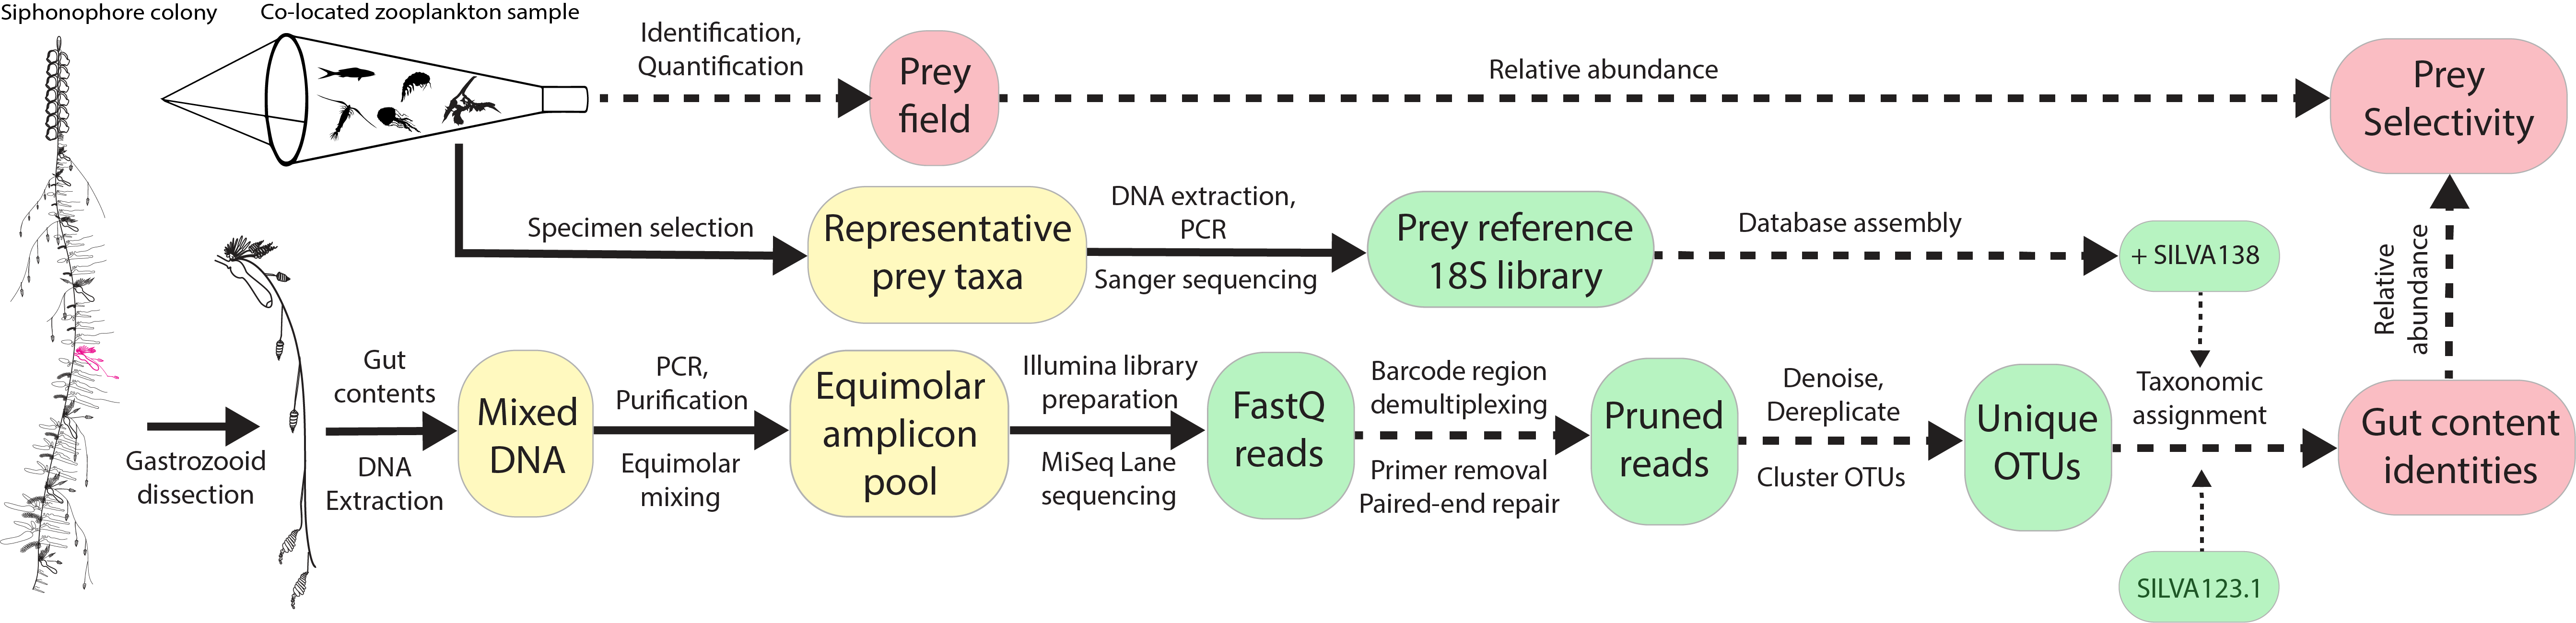
\includegraphics{Figures/methods.png}
\caption{\label{methods_fig} Figure 1. Gut content metabarcoding workflow used in this study. Siphonophore illustrated by Freya Goetz. Silhouettes in the plankton net downloaded from phylopic.org. ``Field'' indicates both processes and concepts at sea. ``Lab'' indicates processes carried out at the molecular bench. ``Cluster'' indicates bioinformatic processes carried out in the supercomputing cluster.}
\end{figure}

Reference database -- In order to enhance the accuracy of the taxonomic assignments of reads, we also built a complementary custom reference 18S gene barcoding database. To do this, we collected 60 specimens of 30 species of zooplankton and micronekton from the OCCE using a mini-tucker trawl net. We targeted species from underrepresented oceanic clades in SILVA databases, including fishes, crustaceans, jellyfishes, urochordates, chaetognaths, polychaetes, and mollusks. Specimens were photographed live, tissue was sampled and frozen, and the rest of the animal was fixed in formalin as a voucher to be identified and preserved at the Yale Peabody Museum of Natural History. DNA extraction, quality control, PCR, and amplicon cleanup was carried out in a similar fashion as the metabarcoding protocol in Damian-Serrano Damian-Serrano (2020), with the exception that only one PCR program was used (Damian-Serrano Damian-Serrano (2020), Table T5A), and only one pair of primers was used (166F and 134R), spanning the full extent of the sequence containing all barcodes used in the gut content metabarcoding (\textasciitilde{}1800bp). Purified amplicons were sent in plates with the forward and reverse primer separately for Sanger sequencing from both ends at the Yale DNA Analysis Facility. These sequences were then trimmed at a 95\% quality cutoff in Geneious, and concatenated with the latest SILVA database (SILVA\_138\_SSURef\_NR99 pruned to remove bacterial sequences) downloaded on February 23rd (2021) to generate our custom-built database.

Bioinformatic pipeline -- Amplicon libraries were demultiplexed by primer sequence using custom bash code. Primer sequences were removed using \emph{cutadapt} (Martin 2011). The forward and reverse reads were matched and repaired using \emph{bbtools} (Bushnell et al. 2017), then denoised and de-replicated using the DADA2 (Callahan et al. 2016) plugin in QIIME2 (Bolyen et al. 2019) with a truncation quality threshold of 28. We \emph{de novo} clustered the unique features into OTUs using the VSEARCH (Rognes et al. 2016) plugin in QIIME2 with a similarity threshold of 95\%. Using QIIME2, we computed sample composition and diversity metrics and aligned the feature sequences with MAFFT (Katoh et al. 2009) to build a phylogenetic tree with Fasttree (Price et al. 2009). To reduce computational load, only the top 100 most abundant features among the clustered OTUs were selected for taxonomic assignment. Taxonomic identifications were assigned using the assignment software METAXA2 (Bengtsson-Palme et al. 2015) with a 70\% reliability cutoff, comparing the sequences against the standard GenBank reference library, the SILVA123.1 reference library {[}quast2012silva{]}, and our custom-built library (based on SILVA138). All bioinformatics analyses were carried out in the Yale High Performance Computing Cluster. The taxonomic assignments and read count data were merged, then parsed to match the sample of origin and the DNA sequence they derived from. Sequence post-processing scripts can be found in the Dryad repository (citation TBD).

Assignment interpretation -- Taxonomic assignments were then manually inspected and annotated with the interpreted consensus taxon and interpreted source (predator, prey, secondary predation, parasite, environmental eukaryote, unrecognizable sequence, contamination, or cross contamination). A combination of annotation database consensus, barcode consensus, number of reads, manual BLAST checks, and natural history informed priors were used to assign these interpretations. Amplification experiments on negative controls indicated that the human, mite, and insect contaminants originated from specimen manipulation in the field and not from the lab bench. Cross-contamination at the lab bench was suspected for some samples in runs 0 and 5 due to simultaneous DNA extractions of potential prey samples. Reads which were suspected of cross-contamination (assigned to taxa present in the potential sources of contamination, present across multiple samples in the same run with very low read abundances) were conservatively labelled as such. Crustacean, gastropod, and larvacean sequences in Physalia samples were interpreted as secondary predation (prey of their fish prey) given our knowledge on the prey-capture limitations of these animals and the feeding habits of fish. When all barcodes except `152' indicate mysid prey but `152' identifies a similar number of reads as stomatopod prey, those reads are interpreted as mysid prey. Assignments of shark identities by barcode `152' in one of the Physalia samples (extraction 169) were identified as ray-finned fish prey on BLAST and interpreted as such, in agreement with the other barcodes. Assignment of decapod crustacean identities by barcode `152' (in extractions 111, 218, and 225) were interpreted as euphausiid prey in agreement with the assignments on the rest of the barcodes. The taxonomic composition of the samples was analyzed and visualized in the R programming environment. Scripts available in Dryad repository (citation TBD).

Prey field characterization -- In order to compare the observed diet to the environmental abundances of potential prey taxa, we collected zooplankton and micronekton samples the same day and location (cruise station coordinates) as the gut content samples they are paired with. The plankton samples paired with epipelagic siphonophore specimens were collected using a weighted hand-held plankton net (ring diameter of 1m for the Bermuda samples, 0.5m for the OCCE samples, mesh size of 250µm) towed for \textasciitilde{}10min at a few meters under the surface at a speed of \textasciitilde{}1kt. Paired with the ROV-collected mesopelagic siphonophore specimens, we collected macroplankton and micronekton samples using a mini-tucker trawl net (frame area: 2m\textsuperscript{2}, mesh size: 500µm) towed for \textasciitilde{}2h between 900m and the surface at night. Environmental community samples were visually examined live to collect specimens to sequence for the 18S reference library and other purposes, which were annotated as removed. Samples were concentrated using metal sieves and fixed in 4\% formalin. Back in the Yale Peabody Museum of Natural History, these samples were visually identified and quantified from a splitter aliquot. In order to estimate how selective siphonophore species are for different prey types in the environment, we calculated Strauss Strauss (1979) Linear Index (LI).

Comparisons to published sources -- In this study we aim to compare the results of DNA metabarcoding of gut contents to those from submersible observations and visual gut content inspections. Therefore, we used the dietary data compiled in Damian-Serrano et al. Damian-Serrano et al. (2021) from eleven published sources divided into those that used gut content inspections and those that used submersible observations. Salps, ctenophores, and medusae were merged into a gelatinous prey concept for comparative purposes. Published records for \emph{Apolemia uvaria} were considered equivalent to \emph{Apolemia} sp. for genus level comparisons. Records of all \emph{Forskalia} species were considered equivalent to \emph{Forskalia} sp. In order to test the morphology-based dietary predictions generated in Damian-Serrano et al. Damian-Serrano \& Dunn (2022), we used the Bayesian posterior probabilities for each feeding guild for each species. Small-crustacean guild predictions were mapped to copepod, ostracod, and cladoceran prey concepts. Large-crustacean guild predictions were mapped to decapod, euphausiid, mysid, lophogastrid, stomatopod, and amphipod prey concepts. Generalist guild predictions were mapped to all prey concepts except gelatinous prey (following the intended distinction with gelatinous specialists used in Damian-Serrano et al. Damian-Serrano et al. (2021)).

\hypertarget{results}{%
\subsection*{Results}\label{results}}
\addcontentsline{toc}{subsection}{Results}

We obtained a total of 4148 unique sequences, including 1502 sequences from barcode ``134'', 614 from barcode ``152'', 758 from barcode ``166'', 497 from barcode ``179'', and 341 from barcode ``261'', and 442 from barcode ``272''. A total of 337 unique sequences were interpreted as prey items, 36 as secondary predation, 292 as contamination from extrinsic sources, 2857 as natural environmental DNA sources, 791 as siphonophore sequences, 85 as parasites (myxozoans, trematodes, and other helminths), and 14 unrecognizable sequences.
We extracted, amplified, and sequenced the gut contents of 159 specimens from 41 siphonophore species and identified prey items in 47 specimens from 24 species. We identified 55 prey items, 42 of which were crustaceans (25 of which were copepods). In addition, three of them were fishes, four of them were thaliaceans, five corresponded to other gelatinous predators (ctenophores and a medusae), and one matching to a bivalve mollusc. Most (112 out of 159) siphonophore specimens collected did not yield any putative prey concepts. Among the 47 specimens with prey, 40 of them had DNA from a single prey item, while only six had two prey items, and one \emph{Apolemia} sp. specimen had three prey items (SM Fig. 1). This is consistent with the feeding habits of sit-and-wait ambush predators in oligotrophic environments, with scarce feeding events separated by periods of starvation.

\begin{figure}
\centering
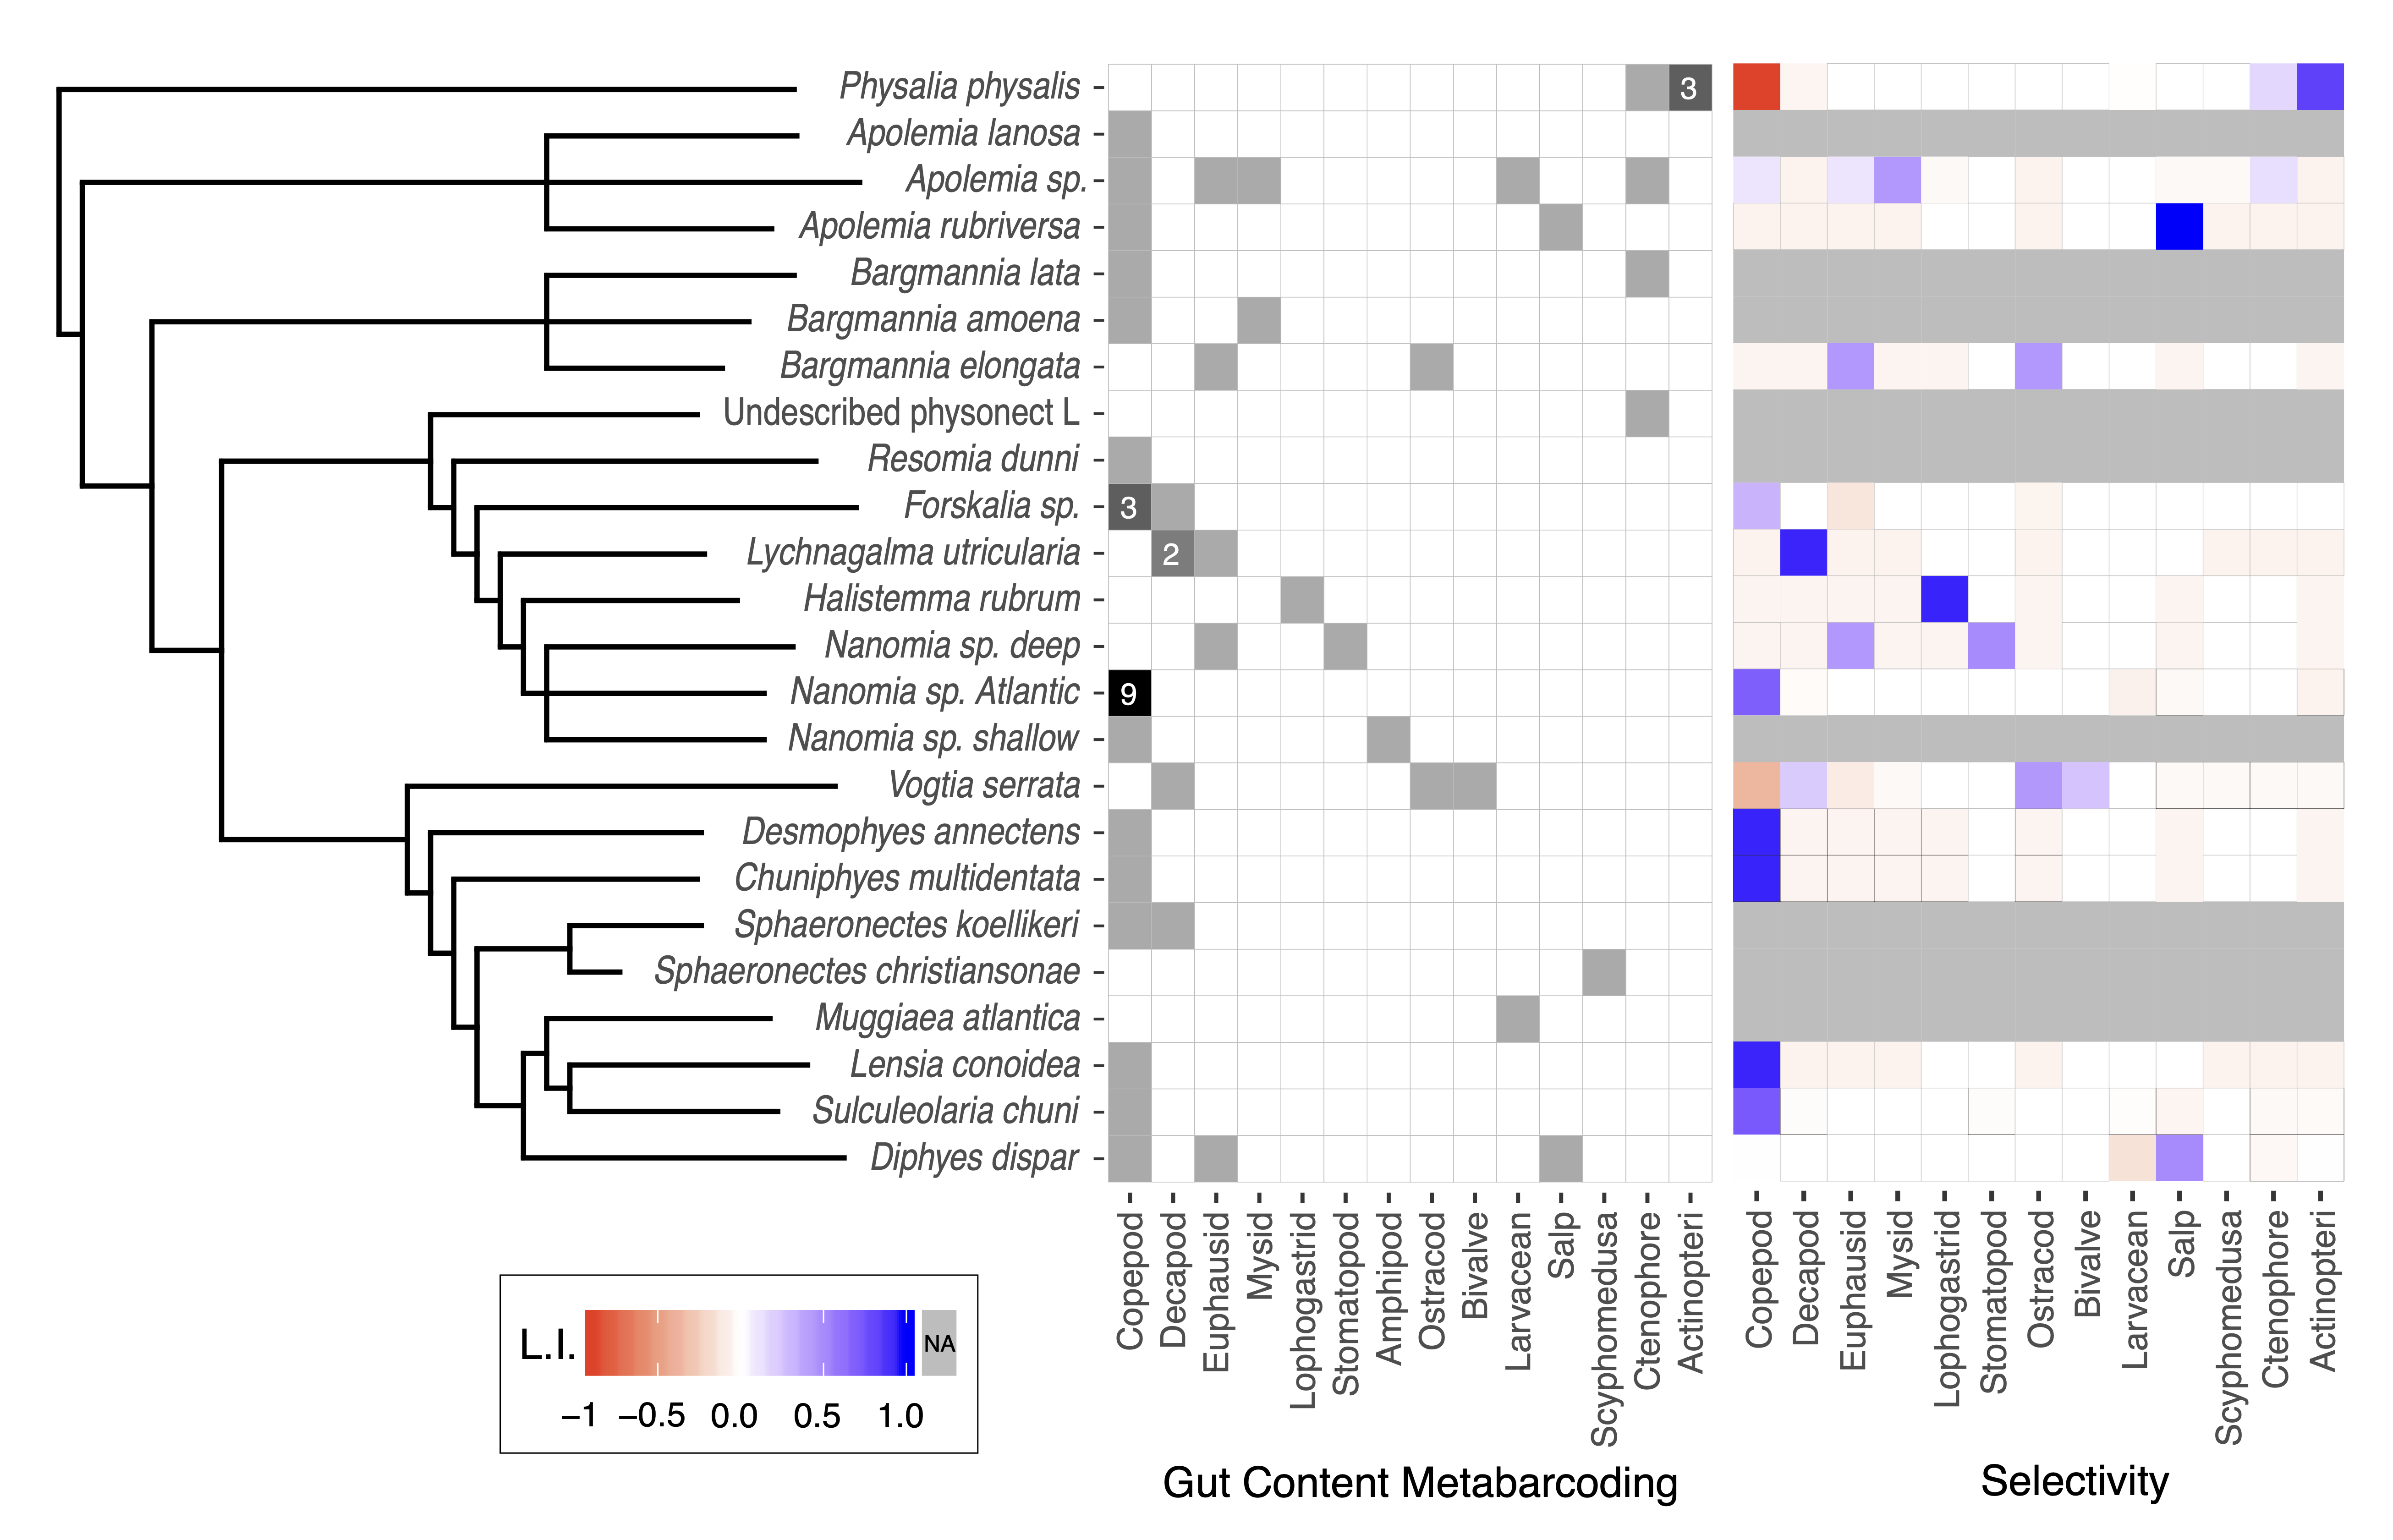
\includegraphics{Figures/GC-SEL_spp.png}
\caption{\label{spp_gcsel} Figure 2. Species-wise grid with the frequency of the major prey types identified from the metabarcoding data (left) and the average prey-type selectivity estimated in comparison with the local planktonic community composition (right). Gut content cells in white indicate absence, and in cells in grey indicate presence in one specimen, or more than one specimen if labeled with a number. Selectivity heatmap mapped to Strauss' L.I. values. Phylogenetic cladogram based on the tree published in Damian-Serrano et al. (2021).}
\end{figure}

When comparing the identified prey to the co-localized prey field, we only find strong negative (\textless{}-0.5) selectivity for copepods in \emph{P. physalis} specimens and in one specimen of \emph{Vogtia serrata}. We do find strong positive selectivity (\textgreater{}0.5) in 19 specimens from 12 species (out of the 15 species assessed). These cases include: selectivity for fish in \emph{Physalia}; selectivity for copepods in \emph{Lensia conoidea}, \emph{Chuniphyes multidentata}, \emph{Desmophyes annectens}, \emph{S. chuni}, and Atlantic \emph{Nanomia} sp.; selectivity for ostracods in \emph{Vogtia serrata}; selectivity for decapods in \emph{Lychnagalma utricularia}, for lophogastrids in \emph{Halistemma rubrum}, and for mysids in \emph{Apolemia} sp.; and selectivity for salps in \emph{Apolemia rubriversa} and \emph{Diphyes dispar} (Fig. @ref(spp\_gcsel)). Comparing our metabarcoding findings with the morphology-based predictions from Damian-Serrano et al. Damian-Serrano \& Dunn (2022), we confirmed 15 predicted interactions between siphonophores and prey. On the other hand, among the species studied there were 70 predicted interactions that were not confirmed by the metabarcoding results (Fig. @ref(source\_comparison)). Out of the 10 taxa with morphology-based predictions and metabarcoding results, six had all prey congruent with the predictions, three had all prey incongruent with the predictions, and \emph{Forskalia} sp. presented both cases.

\begin{figure}
\centering
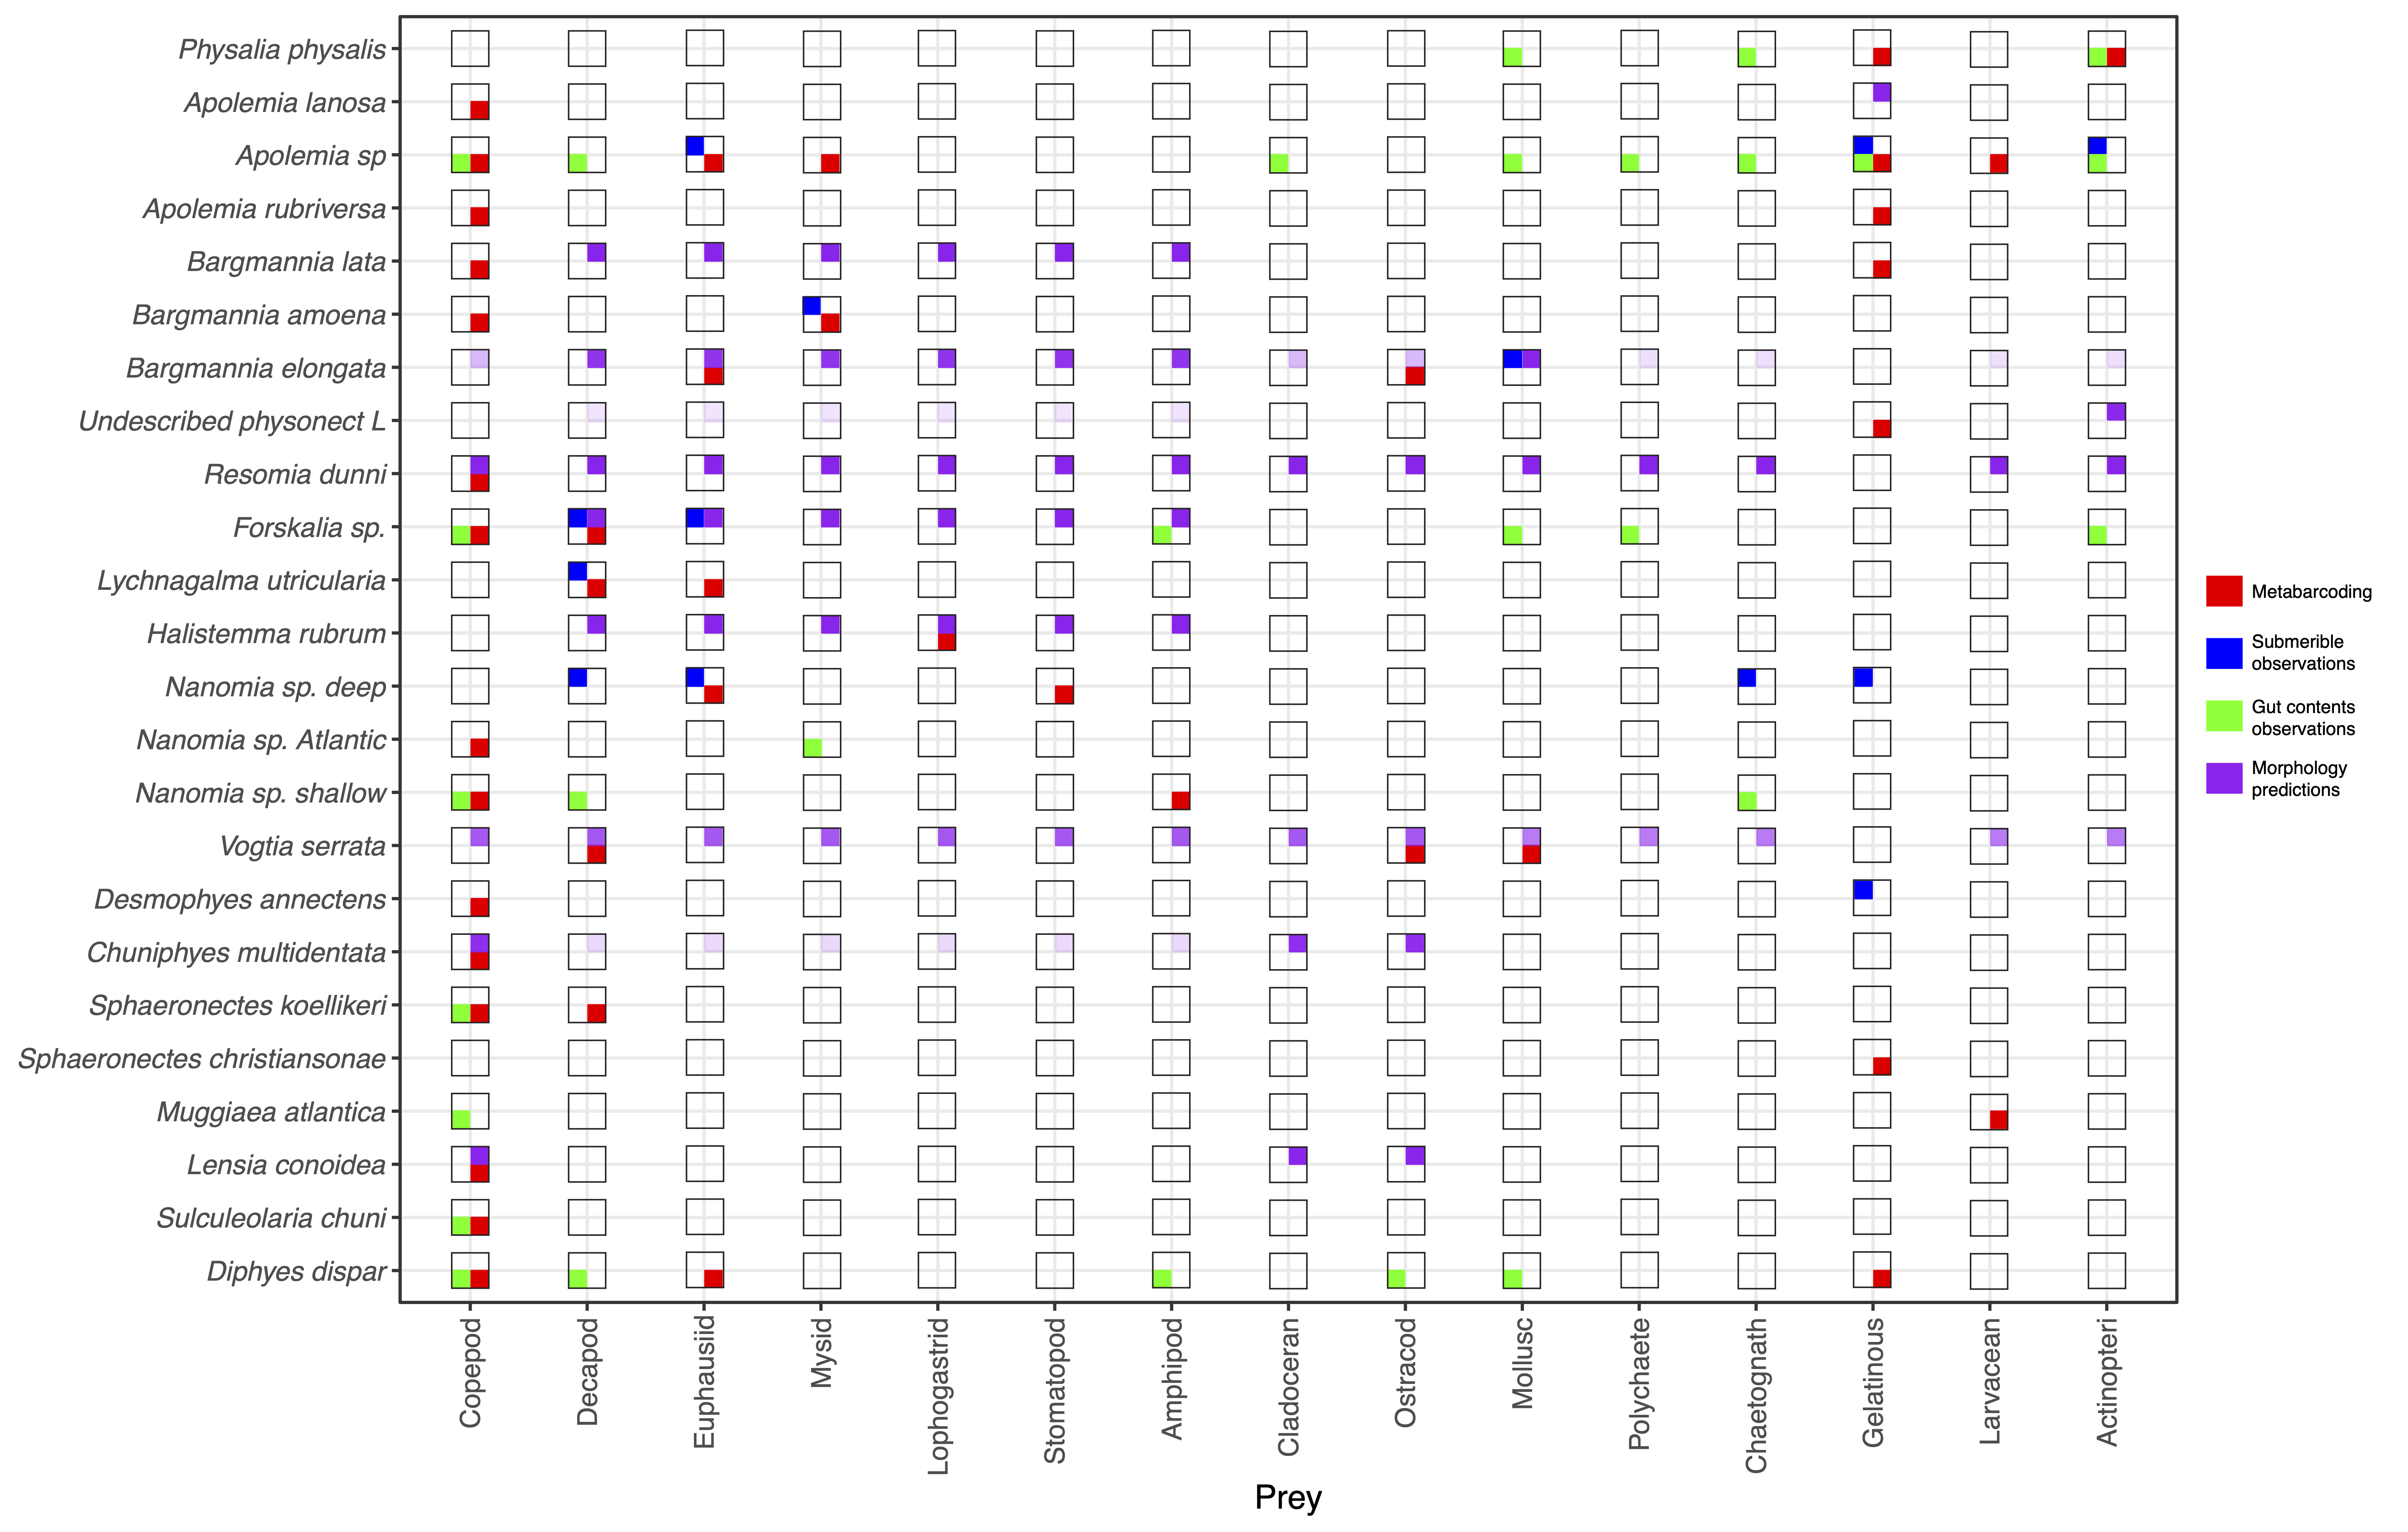
\includegraphics{Figures/Source_comparison.png}
\caption{\label{source_comparison} Figure 3. Feeding interactions between siphonophore species and their prey identified by our metabarcoding results (red), published submersible observations (blue), published visual gut content analyses (green), and predicted by the morphology-based DAPC model in Damian-Serrano et al. (2021).}
\end{figure}

We reported the first insights into the diets of nine siphonophore species, and revealed 29 novel predator-prey interactions (Fig. @ref(source\_comparison)). When comparing our metabarcoding findings with the published visual observations from gut content inspections and submersible dives, we found five interaction congruent with ROV observations, and eight interactions (six of them involving copepods) congruent with visual gut content inspections of SCUBA-collected colonies (Fig. @ref(source\_comparison)). Our novel findings suggest that visual inspections of gut contents may have missed gelatinous prey in \emph{P. physalis}, and potentially missed larvacean prey in \emph{Apolemia} and \emph{Muggiaea atlantica}. In mesopelagic species, we suspect that submersible observations may have missed copepod prey in \emph{Desmophyes annectens}, \emph{Forskalia} sp., and \emph{Apolemia} sp.; ostracod prey in \emph{Bargmannia elongata}; and larvacean prey in \emph{Apolemia} sp.

The Portuguese man-o-war (\emph{P. physalis}) is the only pleustonic (surface floating) member of the siphonophores, and the most commonly encountered by beachgoers. In our gut content samples from Bermuda, we found three specimens with ray-finned fish sequences, some of which had visually recognizable fish in the gastrozooids when collected. Fish prey is congruent with published visual inspections of their gut contents {[}Purcell (1981a);bardi2007taxonomic{]}. In all three specimens with fish prey we also found benthic and hard-bodied taxa (mysid, alpheid shrimp, spider crab, copepod, benthic gastropod, and a sipunculid worm), as well as larvacean sequences. Man-o-wars are well-known to feed exclusively on relatively large and motile soft-bodied prey such as fish, chaetognaths, or pelagic gastropods. Their nematocysts are not able to subdue crustacean prey, and their feeding reflex would not trigger with a prey as small as a larvacean. Therefore, we interpreted the presence of these taxa in the gut contents as secondary predation (prey of the fish prey). In addition, we also detected a ctenophore in the gut contents of one specimen. This could be also a case of secondary predation, but we suspect a ctenophore could be large enough to be prey of the man-o-war. If that is the case, this would be the first record of \emph{Physalia} consuming gelatinous zooplankton, which would place the man-o-war as a central species in the epipelagic `jelly-web' (Chi et al. 2020). Comparisons with their surrounding prey field show these specimens were strongly selective for fish and strongly exclusive of copepods (Fig. @ref(spp\_gcsel)).

\emph{Apolemia} physonects are among the longest siphonophores, with colonies reaching as far as 30m of length. Their tentacles are different from other siphonophores since they have no tentilla, and carry birhopaloid heteroneme nematocysts directly on the tentacles (Damian-Serrano \& Dunn 2022). \emph{Apolemia} species are known to consume all sorts of prey including crustaceans, molluscs, polychaetes, chaetognaths, fish, and gelatinous zooplankton (Purcell 1981a, Choy et al. 2017). While this may suggest these species are generalists, Damian-Serrano et al. Damian-Serrano et al. (2021) hypothesized that they may be gelatinous zooplankton specialists, since they consume a larger proportion of this prey type than other siphonophores, their nematocysts have similar traits to those in other gelativore cnidarians, and their apparent generality could be explained by the sheer number of fine tentacles deployed for prey capture per colony, which would inevitable entangle almost anything that swims by. All species of \emph{Apolemia} analyzed here had consumed copepods, the \emph{A. rubriversa} had also consumed a salp, and the undescribed \emph{Apolemia} species also had ctenophore, larvacean, mysid, and euphausiid prey sequences. The high selectivity of \emph{A. rubriversa} for salp prey is congruent with its characterization as a gelatinous specialist in Damian-Serrano et al. (2021). The morphology-based predictions derived from Damian-Serrano et al. Damian-Serrano \& Dunn (2022) indicate that \emph{A. lanosa} should be a gelatinous prey specialist. This is incongruent with our finding of just copepod prey, but it is possible that the doliolid and hydromedusa reads we conservatively labelled as potential cross-contamination could correspond to real prey. In light of these interspecific differences, it is possible that these coexisting species of midwater \emph{Apolemia} are partitioning their trophic niche by varying the proportion of crustacean versus gelatinous prey they consume.

Another triad of frequently-observed species in the midwaters off Monterey Bay are the \emph{Bargmannia}. These physonects have relatively simple tentilla with large stenotele nematocysts and an undifferentiated terminal filament (Damian-Serrano et al. 2021). ROVs have recorded \emph{B. elongata} consuming crustaceans and cephalopods, during specimen collection we observed a mysid prey in a specimen \emph{B. amoena}, yet nothing was known about the diet of \emph{B. lata}. DNA metabarcoding confirmed the identity of the mysid in \emph{B. amoena} as \emph{Boreomysis californica}, and found a copepod in another specimen. One \emph{B. elongata} specimen had euphausiid and ostracod prey, in agreement with the DAPC prediction for \emph{B. elongata} to feed mainly on large crustaceans, but also marginally on small crustaceans. The two \emph{B. lata} specimens were consuming a ctenophore and a copepod respectively. These results are not congruent with the morphology-based prediction for \emph{B. lata} to be a large-crustacean specialist (Fig. @ref(source\_comparison)). It seems plausible that these three species ecologically differentiate from each other by consuming different crustacean prey, as well as by tapping into the deep `jelly-web' by consuming ctenophore prey.

Other deep-sea physonects also present interesting results. Undescribed physonect sp. L was predicted to be a fish specialist with a secondary affinity for large crustacean prey. However, we found this specimen consuming a ctenophore. \emph{Resomia dunni} was predicted to be a generalist, which is congruent with the copepod prey we found in its gut contents. \emph{Forskalia} species have been observed to consume various crustaceans, molluscs, worms and fish. Morphology predicts \emph{Forskalia} species to be large crustacean specialists. We found three midwater \emph{Forskalia} specimens with copepod prey in the guts, one of them also had consumed a sergestid shrimp. These results are fully congruent with those derived from visual methods, and partly congruent with the morphological predictions. \emph{Lychnagalma utricularia} is unique among the physonects for bearing a medusa-shaped floating vesicle at the end of their large, coiled tentilla. They have been observed through ROVs consuming sergestid shrimp. We found two specimens both with sergestid shrimp prey (for which they are strongly selective), yet one of them was also digesting a euphausiid. This is consistent with their large-crustacean specialization. \emph{Halistemma rubrum}'s tentilla closely resemble those of \emph{Forskalia}, and thus they are also predicted to be large-crustacean specialists. This prediction is congruent with our identification of a lophogastrid in the gut contents for which it was strongly selective.

Nanomia species are among the most common siphonophores in both Atlantic and Pacific waters, both in epipelagic and midwater environments. Midwater ROV observations of deep-dwelling \emph{Nanomia} have predominantly reported interactions with krill prey, as well as with the occasional chaetognath or sergestid. We identified one specimen of mesopelagic Nanomia with krill and stomatopod DNA in its gut contents, in agreement with its large-crustacean specialist characterization. Epipelagic \emph{Nanomia} might not be as specialized on large crustacean prey, since the literature reports a combination of copepod, decapod, mysid, and chaetognath prey. In the North Pacific Ocean, our metabarcoding identified copepod prey in an epipelagic \emph{Nanomia} off California, a hyperiid amphipod prey in an epipelagic \emph{Nanomia} off Hawaii. This amphipod could have been a commensal or parasite on the \emph{Nanomia} instead of prey, though this is unlikely since only the gastrozooids were dissected and amphipods tend to colonize the nectophores or bracts. In the North Atlantic Ocean, we sampled 14 specimens of epipelagic \emph{Nanomia}, seven of which contained copepod prey. Upon visual inspection of the sampled gastrozooids we could identify \emph{Temora}, \emph{Centropages}, and \emph{Acartia} copepods, the most abundant genera in the plankton sample, whose identity was also confirmed by the metabarcoding results. The corresponding environmental plankton samples showed that these waters were dominated by cladocerans, and thus these \emph{Nanomia} were positively selecting for copepod prey and selecting against cladoceran prey (not detected). We have observed that epipelagic \emph{Nanomia} tend to have smaller tentilla than their mesopelagic counterparts, which may account for their specialization on smaller crustaceans (such as copepods) instead of larger crustaceans (such as krill). The exclusion of the overabundant cladocerans from the diet of these \emph{Nanomia} suggests that their specialization could be copepod-specific.

Calycophorans are characterized by their lack of a pneumatophore (gas-filled apical vesicle) and their structurally homogeneous tentilla Damian-Serrano \& Dunn (2022). However, these tentilla present a great variation in nematocyst number and size, which may translate into dietary differences. \emph{Vogtia} is the closest relative to \emph{Hippopodius}, the only siphonophore known to be an ostracod specialist (Purcell 1981a). Like many other hard-to-access mesopelagic taxa, the diet of \emph{Vogtia} has remained unknown, though tentilla morphology predicts them to be generalists (Damian-Serrano \& Dunn 2022). Pugh Pugh (1986) found spatial correlations between ostracods and \emph{Vogtia} species, and even mentions a \emph{Vogtia} sp. specimen which had the exoskeleton of an ostracod in its gut contents. Our DNA metabarcoding on \emph{V. serrata} has revealed one specimen feeding on an ostracod, and a specimen feeding on a sergestid shrimp and a bivalve. These results are consistent with the generalist morphological prediction, and congruent with the single visual finding of an ostracod in a congener from Pugh Pugh (1986). The presence of an ostracod and a bivalve (likely a veliger larva), which has a very similar shape to an ostracod (with two hard valves), indicates phylogenetic conservatism of diet within Hippopodidae. This is also supported by the fact that the ostracod capture appears to be highly selective given the corresponding community composition.

We provided the first insights into the diets of two extremely abundant deep-sea calycophorans, \emph{Lensia conoidea} and \emph{Chuniphyes multidentata}, which morphology predicted as small-crustacean specialists. Both sequenced specimens had copepod DNA, confirming these predictions. Gelatinous prey has been reported for calycophorans (such as \emph{Praya dubia} or \emph{Desmophyes annectens}) from ROV observations. We report the first instance of gelatinous prey in \emph{Diphyes dispar} (salp prey), \emph{M. atlantica} (larvacean), and \emph{Sphaeronectes christiansonae} (nausithoid medusa). The latter constitutes the first record of \emph{S. christiansonae} feeding, though the minute size of this predator renders this interaction dubious. The far more common epipelagic \emph{Sphaeronectes} species, \emph{S. koellikeri}, appears to be a copepod specialist according to visual gut content analysis (Purcell 1981a). We sequenced the gut contents of two specimens of this species, one of them indeed was consuming a copepod, yet the other was consuming a crab larva, which constitutes a novel prey type for this species, while still within the expected range of a small-crustacean specialist. Another confirmed expectation occurred with \emph{S. chuni,} a visually-assessed copepod specialist in Purcell Purcell (1981a), for which we detected a copepod prey in an Atlantic specimen.

\hypertarget{discussion}{%
\subsection*{Discussion}\label{discussion}}
\addcontentsline{toc}{subsection}{Discussion}

This study constitutes the first use of DNA metabarcoding for siphonophore gut contents, as well as the first application of this technology to investigate the diets of marine gelatinous predators. Our results expand the existing knowledge on siphonophore diets, detecting prey types previously missed by visual methods, and providing the first insights into the diets of several understudied siphonophore species. By comparing the taxonomic composition of the gut contents to that of the environmental planktonic community, we confirm that most of the examined siphonophore species are strongly selective specialists. Moreover, we find that many of the tentilla morphology-based dietary predictions for these species were confirmed by the metabarcoding results. We show that whole gastrozooids can be utilized for DNA metabarcoding of diets without need for further dissection nor the use of predator blocking primers.
We identified representatives from sixteen animal phyla among the gut contents studied, six among the identified prey items (SM2-5). This shows the phylogenetic range of taxa that can be amplified with our primer pairs. Overall, crustaceans (especially copepods) were identified as the most frequent prey type among siphonophore diets. Copepods are typically the most abundant prey type in planktonic communities, thus being able to feed on them is an advantageous strategy for any planktivorous predator. Fish prey were detected only in the Portuguese man-o-war samples, in agreement with most published observations of man-o-war feeding. For most siphonophore species assessed herein, their prey belonged to the rarer components of the planktonic community, demonstrating high prey selectivity. However, the selectivity index values presented in this study should be interpreted with care, since the prey field data is quantitative but the gut content presences are only binary.

We have detected prey types previously missed by visual methods (microscopic gut content observations and submersible observations) such as larvaceans, ctenophores, bivalves, and ostracods. These results are consistent with the hypothesis that small prey is underestimated in submersible observations and rapidly-digested prey is underestimated by gut content inspections. DNA metabarcoding was able to detect prey both small and large, gelatinous and hard-bodied, for both deep and shallow-dwelling species. In Damian-Serrano et al. Damian-Serrano \& Dunn (2022) we predicted the diets of understudied siphonophore species based on the morphology of their tentilla and nematocysts. We were able to test these predictions for ten species, and found that most of the prey items found were congruent with these predictions, indicating that tentilla morphology is a strong predictor of siphonophore diets.

Our findings are congruent with the idea that most epipelagic and mesopelagic siphonophore species are strongly selective and specialized predators. Different species were found consuming prey across low (salps, copepods, ostracods) and high (fish, ctenophores, medusae) trophic levels. In addition, finding of larvaceans and salps in the diets of four species should shift our perspective on the role of siphonophores in open ocean food-webs, as they may be able to directly feed filter-feeding prey at lower trophic levels, placing some species one trophic level away from phytoplankton productivity and the microbial loop.

While DNA-based tools can detect prey unrecognized by visual methods, they are not free of shortcomings. Since all life stages of an animal have the same genetic signature, metabarcoding tools are unable to distinguish between larval, juvenile, or adult prey. These ontogenetic stages can have vastly different ecological implications and pose radically different challenges during prey capture. In addition, the application of metabarcoding to predator diets is usually not quantitative, since too many sources of variation may lead to differences in read abundance. For example, different animal phyla have different sizes, cell densities (due to variable acellular mesoglea content), digestion rates {[}Deagle \& Tollit (2007) ;Troedsson et al. (2009);valentini2009new{]}, number of copies of the target gene, or primer affinities during the PCR. Due to the difficulties inherent to locating and sampling the species examined in this study, frequency-based quantitative comparisons were not possible either.

Siphonophores differ from other consumers in several ways which impose further limitations to the value of gut content metabarcoding. The most important difference is the feeding mode and feeding rate, especially for deep-sea species, which typically consume one prey at a time and do not get a chance to capture another until far after the former has been digested (Mackie et al. 1988). Therefore, most siphonophores are found with empty guts or digesting one or few prey items at a time. Thus the sample size required for frequency-based analyses is much higher than for other consumers which feed more frequently. Our prey frequency results are consistent with this idea. Moreover, excepting some siphonophores, such as \emph{Rhizophysa} and \emph{Rosacea} which are diurnal feeders (Purcell 1981a), most species also feed during the night. In the open ocean, diel vertical migration drastically changes the prey field composition for siphonophores at night. Given the fieldwork limitations in this study, we were only able to collect siphonophore gut contents during the day, thus biasing their diet towards their diurnal prey captures.

Overall, this investigation was successful in demonstrating the suitability and effectiveness of DNA metabarcoding to identify the prey consumed by siphonophores from gastrozooid contents, providing novel insights into the ecology and natural history of several siphonophore species, assessing prey selectivity in comparison with their prey-field, assessing the biases in visual prey detection methods, and validating the power of tentilla morphology to predict siphonophore diets. We find that siphonophores are specialized and selective predators which have diversified their feeding habits to consume fish, crustaceans, gelatinous predators, filter-feeders, meroplanktonic larvae, and other pelagic invertebrates.

\hypertarget{acknowledgements}{%
\subsection*{Acknowledgements}\label{acknowledgements}}
\addcontentsline{toc}{subsection}{Acknowledgements}

We would like to thank Gisella Caccone, Carol Mariani, and T.J. Johnson for the Yale DNA Analysis Facility for their invaluable training and their assistance on this study, as well as the staff of the Yale Center for Genomic Analyses for helping us design the sequencing strategy for this study. We also wish to thank Bianca R. Brown for her assistance designing the read processing pipeline and Johan Begtsson-Palme for his help troubleshooting our usage of METAXA2. We are grateful to the crew of the R/V Western Flyer, the R/V Kilo Moana, and Jeff Godfrey for making the collection of these samples possible.

\hypertarget{references}{%
\subsection*{References}\label{references}}
\addcontentsline{toc}{subsection}{References}

\hypertarget{refs}{}
\leavevmode\hypertarget{ref-bengtsson2015metaxa2}{}%
Bengtsson-Palme J, Hartmann M, Eriksson KM, Pal C, Thorell K, Larsson DGJ, Nilsson RH (2015) METAXA2: Improved Identification and Taxonomic Classification of Small and Large Subunit rRNA in Metagenomic Data. Molecular ecology resources 15:1403--1414.

\leavevmode\hypertarget{ref-biggs1977field}{}%
Biggs DC (1977) Field Studies of Fishing, Feeding, and Digestion in Siphonophores. Marine \& Freshwater Behaviour \& Phy 4:261--274.

\leavevmode\hypertarget{ref-bolyen2019reproducible}{}%
Bolyen E, Rideout JR, Dillon MR, Bokulich NA, Abnet CC, Al-Ghalith GA, Alexander H, Alm EJ, Arumugam M, Asnicar F, others (2019) Reproducible, Interactive, Scalable and Extensible Microbiome Data Science Using Qiime 2. Nature biotechnology 37:852--857.

\leavevmode\hypertarget{ref-bushnell2017bbmerge}{}%
Bushnell B, Rood J, Singer E (2017) BBMerge--Accurate Paired Shotgun Read Merging via Overlap. PloS one 12:e0185056.

\leavevmode\hypertarget{ref-callahan2016dada2}{}%
Callahan BJ, McMurdie PJ, Rosen MJ, Han AW, Johnson AJA, Holmes SP (2016) DADA2: High-Resolution Sample Inference from Illumina Amplicon Data. Nature methods 13:581--583.

\leavevmode\hypertarget{ref-chi2020tackling}{}%
Chi X, Dierking J, Hoving H-J, Lüskow F, Denda A, Christiansen B, Sommer U, Hansen T, Javidpour J (2020) Tackling the Jelly Web: Trophic Ecology of Gelatinous Zooplankton in Oceanic Food Webs of the Eastern Tropical Atlantic Assessed by Stable Isotope Analysis. Limnology and Oceanography.

\leavevmode\hypertarget{ref-choy2017deep}{}%
Choy CA, Haddock SH, Robison BH (2017) Deep Pelagic Food Web Structure as Revealed by in Situ Feeding Observations. Proceedings of the Royal Society B: Biological Sciences 284:20172116.

\leavevmode\hypertarget{ref-clarke2018dna}{}%
Clarke LJ, Trebilco R, Walters A, Polanowski AM, Deagle BE (2018) DNA-Based Diet Analysis of Mesopelagic Fish from the Southern Kerguelen Axis. Deep Sea Research Part II: Topical Studies in Oceanography.

\leavevmode\hypertarget{ref-connell2014dna}{}%
Connell S, O'Rorke R, Jeffs A, Lavery S (2014) DNA Identification of the Phyllosoma Diet of Jasus Edwardsii and Scyllarus Sp. Z. New Zealand Journal of Marine and Freshwater Research 48:416--429.

\leavevmode\hypertarget{ref-damianserrano2020dna}{}%
Damian-Serrano A (2020) DNA Metabarcoding Protocol for Siphonophore Gut Contents. protocolsio https://wwwprotocolsio/view/dna-metabarcoding-protocol-for-siphonophore-gut-co-bd8ci9sw.

\leavevmode\hypertarget{ref-damian2021evolution}{}%
Damian-Serrano A, Haddock SH, Dunn CW (2021) The Evolution of Siphonophore Tentilla for Specialized Prey Capture in the Open Ocean. Proceedings of the National Academy of Sciences 118.

\leavevmode\hypertarget{ref-damianserrano2022evolutionary}{}%
Damian-Serrano H Alejandro, Dunn CW (2022) The Evolutionary History of Siphonophore Tentilla: Novelties, Convergence, and Integration. Integrative and comparative biology (in review).

\leavevmode\hypertarget{ref-deagle2007quantitative}{}%
Deagle BE, Tollit DJ (2007) Quantitative Analysis of Prey Dna in Pinniped Faeces: Potential to Estimate Diet Composition? Conservation Genetics 8:743--747.

\leavevmode\hypertarget{ref-fernandez2018predatory}{}%
Fernández-Álvarez FÁ, Machordom A, Garcı'a-Jiménez R, Salinas-Zavala CA, Villanueva R (2018) Predatory Flying Squids Are Detritivores During Their Early Planktonic Life. Scientific Reports 8:1--12.

\leavevmode\hypertarget{ref-haddock2004golden}{}%
Haddock SH (2004) A Golden Age of Gelata: Past and Future Research on Planktonic Ctenophores and Cnidarians. Hydrobiologia 530:549--556.

\leavevmode\hypertarget{ref-haddock2005scientific}{}%
Haddock SH, Heine JN (2005) Scientific blue-water diving. California Sea Grant College Program.

\leavevmode\hypertarget{ref-harbison1992gelatinous}{}%
Harbison GR (1992) The Gelatinous Inhabitants of the Ocean Interior. Oceanus 35:18--23.

\leavevmode\hypertarget{ref-harms2016use}{}%
Harms-Tuohy CA, Schizas NV, Appeldoorn RS (2016) Use of Dna Metabarcoding for Stomach Content Analysis in the Invasive Lionfish Pterois Volitans in Puerto Rico. Marine Ecology Progress Series 558:181--191.

\leavevmode\hypertarget{ref-hetherington2021moving}{}%
Hetherington E, Haddock A Damian-Serrano, Choy A (2021) Moving beyond medusae: Integrating siphonophores into marine food web ecology. In: \emph{Limnology and Oceanography Letters}. Wiley Online Library

\leavevmode\hypertarget{ref-jensen2018tracing}{}%
Jensen MR, Knudsen SW, Munk P, Thomsen PF, Møller PR (2018) Tracing European Eel in the Diet of Mesopelagic Fishes from the Sargasso Sea Using Dna from Fish Stomachs. Marine Biology 165:1--11.

\leavevmode\hypertarget{ref-katoh2009multiple}{}%
Katoh K, Asimenos G, Toh H (2009) Multiple alignment of dna sequences with mafft. In: \emph{Bioinformatics for dna sequence analysis}. Springer, pp 39--64

\leavevmode\hypertarget{ref-kearse2012geneious}{}%
Kearse M, Moir R, Wilson A, Stones-Havas S, Cheung M, Sturrock S, Buxton S, Cooper A, Markowitz S, Duran C, others (2012) Geneious Basic: An Integrated and Extendable Desktop Software Platform for the Organization and Analysis of Sequence Data. Bioinformatics 28:1647--1649.

\leavevmode\hypertarget{ref-lapides2021prey}{}%
Lapides D-S Alexandra, others (2021) Prey Selectivity and Dietary Specialization in Midwater Siphonophores Based on Rov Observations. in prep.

\leavevmode\hypertarget{ref-leray2013new}{}%
Leray M, Yang JY, Meyer CP, Mills SC, Agudelo N, Ranwez V, Boehm JT, Machida RJ (2013) A New Versatile Primer Set Targeting a Short Fragment of the Mitochondrial Coi Region for Metabarcoding Metazoan Diversity: Application for Characterizing Coral Reef Fish Gut Contents. Frontiers in zoology 10:1--14.

\leavevmode\hypertarget{ref-mackie1988siphonophore}{}%
Mackie G, Pugh P, Purcell J (1988) Siphonophore Biology. Advances in Marine biology 24:97--262.

\leavevmode\hypertarget{ref-mapstone2014global}{}%
Mapstone GM (2014) Global Diversity and Review of Siphonophorae (Cnidaria: Hydrozoa). PLoS One 9:e87737.

\leavevmode\hypertarget{ref-marques2019molecular}{}%
Marques R, Darnaude AM, Crochemore S, Bouvier C, Bonnet D (2019) Molecular Approach Indicates Consumption of Jellyfish by Commercially Important Fish Species in a Coastal Mediterranean Lagoon. Marine environmental research 152:104787.

\leavevmode\hypertarget{ref-martin2011cutadapt}{}%
Martin M (2011) Cutadapt Removes Adapter Sequences from High-Throughput Sequencing Reads. EMBnet journal 17:10--12.

\leavevmode\hypertarget{ref-mcinnes2017high}{}%
McInnes JC, Alderman R, Lea M-A, Raymond B, Deagle BE, Phillips RA, Stanworth A, Thompson DR, Catry P, Weimerskirch H, others (2017) High Occurrence of Jellyfish Predation by Black-Browed and Campbell Albatross Identified by Dna Metabarcoding. Molecular Ecology 26:4831--4845.

\leavevmode\hypertarget{ref-price2009fasttree}{}%
Price MN, Dehal PS, Arkin AP (2009) FastTree: Computing Large Minimum Evolution Trees with Profiles Instead of a Distance Matrix. Molecular biology and evolution 26:1641--1650.

\leavevmode\hypertarget{ref-pugh1986trophic}{}%
Pugh P (1986) Trophic Factors Affecting the Distribution of Siphonophores in the North Atlantic Ocean. UNESCO Technical Papers in Marine Science 49:230--234.

\leavevmode\hypertarget{ref-purcell1981dietary}{}%
Purcell J (1981a) Dietary Composition and Diel Feeding Patterns of Epipelagic Siphonophores. Marine Biology 65:83--90.

\leavevmode\hypertarget{ref-purcell1981feeding}{}%
Purcell JE (1981b) Feeding Ecology of Rhizophysa Eysenhardti, a Siphonophore Predator of Fish Larvae 1. Limnology and Oceanography 26:424--432.

\leavevmode\hypertarget{ref-van2018preliminary}{}%
Reis AL van der, Laroche O, Jeffs AG, Lavery SD (2018) Preliminary Analysis of New Zealand Scampi (Metanephrops Challengeri) Diet Using Metabarcoding. PeerJ 6:e5641.

\leavevmode\hypertarget{ref-robison2004deep}{}%
Robison BH (2004) Deep Pelagic Biology. Journal of experimental marine biology and ecology 300:253--272.

\leavevmode\hypertarget{ref-rognes2016vsearch}{}%
Rognes T, Flouri T, Nichols B, Quince C, Mahé F (2016) VSEARCH: A Versatile Open Source Tool for Metagenomics. PeerJ 4:e2584.

\leavevmode\hypertarget{ref-strauss1979reliability}{}%
Strauss RE (1979) Reliability Estimates for Ivlevˈs Electivity Index, the Forage Ratio, and a Proposed Linear Index of Food Selection. Transactions of the American Fisheries Society 108:344--352.

\leavevmode\hypertarget{ref-troedsson2009quantification}{}%
Troedsson C, Simonelli P, Nägele V, Nejstgaard JC, Frischer ME (2009) Quantification of Copepod Gut Content by Differential Length Amplification Quantitative Pcr (Dla-qPCR). Marine Biology 156:253--259.


\end{document}
